\documentclass[10pt, titlepage, oneside, a4paper]{article}
\usepackage[T1]{fontenc}
\usepackage[UKenglish]{babel}
\usepackage[UKenglish]{isodate}
\usepackage{algorithm2e}
\usepackage{hyperref}
\usepackage{tikz}
\usetikzlibrary{shapes.geometric, arrows}
\usepackage[margin=2cm]{caption}
\usepackage[utf8]{inputenc}
\usepackage{amssymb, graphicx, fancyhdr}
\usepackage{mathrsfs,amsmath}
\usepackage{mathtools}
\usepackage{listings}
\usepackage{color}
\usepackage{float}
\usepackage{epsf}
\usepackage{qtree}
\addtolength{\textheight}{20mm}
\addtolength{\voffset}{-5mm}
\renewcommand{\sectionmark}[1]{\markleft{#1}}

\newcommand{\Section}[1]{\section{#1}\vspace{-8pt}}
\newcommand{\Subsection}[1]{\vspace{-4pt}\subsection{#1}\vspace{-8pt}}
\newcommand{\Subsubsection}[1]{\vspace{-4pt}\subsubsection{#1}\vspace{-8pt}}

\newcommand{\mylistings}{\hspace{16px}\lstinputlisting[basicstyle=\ttfamily, numbers=left]}

\newcounter{appendixpage}
\newenvironment{appendices}{
    \setcounter{appendixpage}{\arabic{page}}
    \stepcounter{appendixpage}
}{
}

\newcommand{\appitem}[2]{
    \stepcounter{section}
    \addtocontents{toc}{\protect\contentsline{section}{\numberline{\Alph{section}}#1}{\arabic{appendixpage}}}
    \addtocounter{appendixpage}{#2}
}

\newcommand{\appsubitem}[2]{
    \stepcounter{subsection}
    \addtocontents{toc}{\protect\contentsline{subsection}{\numberline{\Alph{section}.\arabic{subsection}}#1}{\arabic{appendixpage}}}
    \addtocounter{appendixpage}{#2}
}

\newcommand{\matlablistings}{
    \hspace{16px}\lstinputlisting[language=matlab, commentstyle=\color{mygray}, basicstyle=\ttfamily\scriptsize, numbers=left]}

\definecolor{mygreen}{rgb}{0,0.6,0}
\definecolor{mygray}{rgb}{0.6,0.6,0.6}
% \definecolor{mygray}{rgb}{0.5,0.5,0.5}
\definecolor{mymauve}{rgb}{0.58,0,0.82}



\def\inst{Computing Science}
\def\typeofdoc{Project report}
\def\course{Distributed Systems 7.5 Credits}
\def\pretitle{5DV147 - Project}
\def\title{Group communication}
\def\name{Adam Dahlgren, Benjamin Sientzoff}
\def\username{\{dali, ens15bsf\}}
\def\email{\username{}@cs.umu.se}
\def\path{edu/5dv147/project/}
\def\graders{P-O \"{O}stberg, Ewnetu Bayuh Lakew}

\def\fullpath{\raisebox{1pt}{$\scriptstyle \sim$}\username/\path}

\begin{document}

    \begin{titlepage}
        \thispagestyle{empty}
        \begin{large}
            \begin{tabular}{@{}p{\textwidth}@{}}
                \textbf{UME\AA \ \ UNIVERSITY \hfill \today} \\
                \textbf{Department of \inst} \\
                \textbf{\typeofdoc} \\
            \end{tabular}
        \end{large}
        \vspace{10mm}
        \begin{center}
            \LARGE{\pretitle} \\
            \huge{\textbf{\course}}\\
            \vspace{10mm}
            \LARGE{\title} \\
            \vspace{15mm}
            \begin{large}
                \begin{tabular}{ll}
                    \textbf{Name} & \name \\
                    \\
                    \textbf{E-mail} & \texttt{\email} \\
                    \\
                    \textbf{Path} & \texttt{\fullpath} \\
                    \\
                    \textbf{Run} & \texttt{\$ cd bin \&\& ./nameserver.sh (compile)} \\
                                  & \texttt{\$ cd bin \&\& ./chat.sh (compile)} \\
                \end{tabular}
            \end{large}
            \vfill
            \large{\textbf{Grading}}\\
            \mbox{\large{\graders}}
        \end{center}
    \end{titlepage}

    \lfoot{\footnotesize{A. Dahlgren}}
    \rfoot{\footnotesize{\today}}
    \lhead{\sc\footnotesize\title}
    \rhead{\nouppercase{\sc\footnotesize\leftmark}}
    \pagestyle{fancy}
    \renewcommand{\headrulewidth}{0.2pt}
    \renewcommand{\footrulewidth}{0.2pt}

    \newpage

    \pagenumbering{arabic}

    \setlength{\parindent}{0pt}
    \setlength{\parskip}{10pt}

    	\Section{Introduction}
		\paragraph{}{
    Group communication and management is a central part of distributed systems.
This report accounts for the development of \texttt{Gcom}, a middleware that can be used to facilitate group communication as realized in a distributed chat application.
}

\begin{figure}[hb]
	\begin{center}
		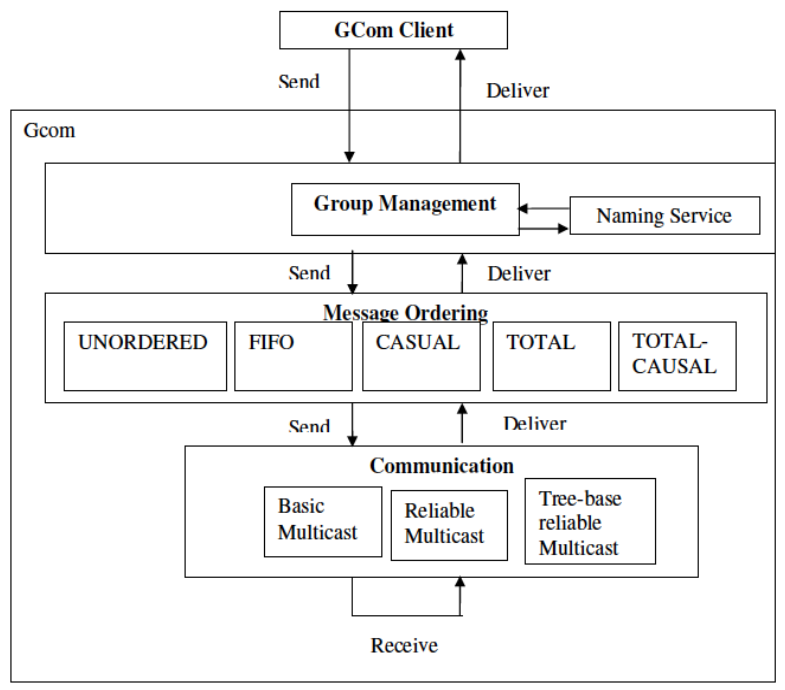
\includegraphics[width=\textwidth]{figures/gcom_intro.png}
	\end{center}
	\caption{
		Overview of the Gcom architecture as given in specification
		\label{fig:gcom_spec}
	}
\end{figure}

\paragraph{}{
Group communication can be broken down to three main modules; Group management, message ordering and communication. These three are layered as shown in Figure \ref{fig:gcom_spec}. For each of these layers there are different algorithms and approaches as to how they function and what behaviour they provide.
Different applications are dependent on different underlying algorithms which means that a group communication middleware should provide easily chosen behaviours in order to be usable.
Gcom is a peer to peer system where all peers have the same responsibility.
}


	\Section{User manual}
		% Meta-info: Java version, build environment, RMI
\subsection{Environment}
\paragraph{}{
    To build the Gcom project, you need a working distribution of maven, java
 1.7 or above. Some scripts are available in the \texttt{bin}, assuming
 you use bash.
}


% Building JAR
\subsection{Compiling Gcom}
\paragraph{}{
    To use the Gcom artifact, you need to compile and package it. To do so,
 just run \texttt{\$ mvn package} in the Gcom folder. The sub-directory
 \texttt{target} may now contain two jar files, \texttt{Gcom-4.2.jar} and
 \texttt{Gcom-4.2-jar-with-dependencies.jar}. The first one can be imported
 to a new project and can be used as a library. The second jar file is the 
 project packed with all needed dependencies and can be use to run directly
 the name server needed by Gcom.
}

% Starting nameserver
\subsection{Name Server}
\paragraph{}{
    To r
}

% Demo chat-app description
\subsection{Gchat, the toy demo of Gcom}
\paragraph{}{
    To show off and prove Gcom works, we build a demonstration application,
 Gchat. It is basically a chat build on top of Gcom.
}

\begin{figure}[h]
    \begin{center}
        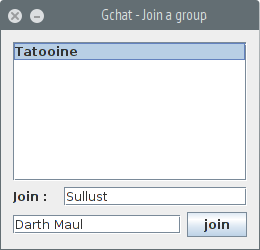
\includegraphics[scale=0.6]{figures/gchat_connection.png}
    \end{center}
    \caption{Connection window of gchat}
    \label{fig:gchat_connect}
\end{figure}

\paragraph{}{
    The application can be found in the sub-directory \texttt{Gchat}. 
 A script in the \texttt{bin} directory allow you to run the application easily
 by running \texttt{chat.sh}. If need, the application can be (re)compiled by 
 giving \texttt{compile} as an argument of the application. Finally you can run
 the debug mode by adding \texttt{debug} to the arguments.
}

\begin{figure}[h]
    \begin{center}
        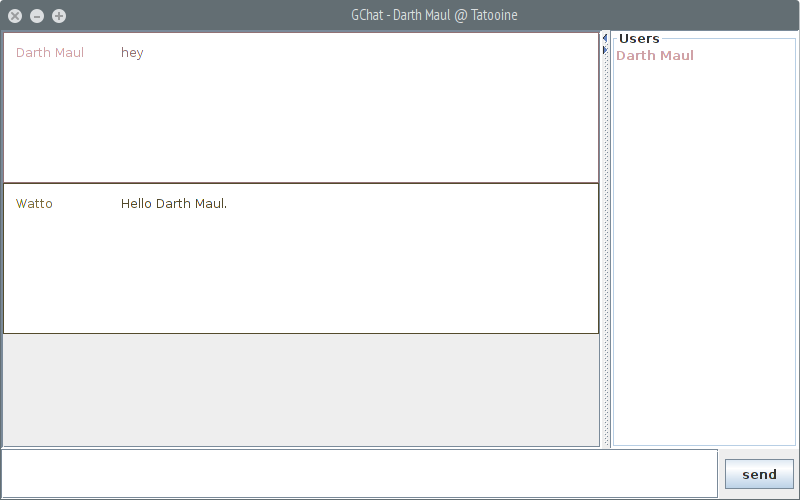
\includegraphics[scale=0.4]{figures/gchat_chat.png}
    \end{center}
    \caption{Chat window of gchat}
    \label{fig:gchat_connectchat}
\end{figure}


% Starting client and creating or joining group

% Further dev 
	% Create own application using Gcom
	
\begin{figure}[h]
    \begin{center}
        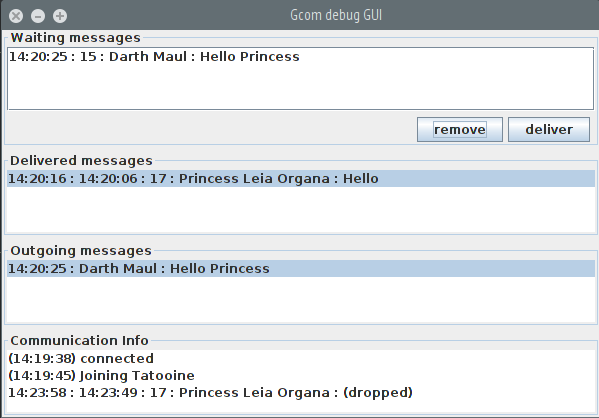
\includegraphics[scale=0.5]{figures/debug_window.png}
    \end{center}
    \caption{Debug interface of Gcom}
    \label{fig:debugGui}
\end{figure}

% trouble shooting ?
\subsection{Trouble shooting}
\paragraph{}{
    The main problem you can get may concern the name server.
}


	
	\Section{Assumptions and limitations}
		There are a couple of limitations to the Gcom middleware as well as the example Gchat applications.
This section covers some of them.

\Subsection{Heartbeat}
	One big limitation of the Gcom middleware is that it does not implement a feature for maintainence of the group, reporting and handling crashed members and similar problems.
	What is done in the current implementation is that whenever a member is found nonrespondant (e.g. when someone sends it a message) this member is reported as crashed and removed from everyones view.
	If it was the leader, an election is initiated.
	One problem with this is that an inactive group the leader can crash and render the group unavailable via the nameserver which in turn lets a joining member start a new group with the same name.
	A solution to this problem would be to implement a heartbeat that periodically polls the entire group for crashed members and handles accordingly.

\Subsection{Network partitioning}
	Network partitioning, when a network is split into more than one piece, is one of the more difficult problems to recover from.
	If this happens to a group in Gcom the two or more subgroups will continue to function but once the network is joined together it is currently not possible to reconstruct the original group correctly.

\Subsection{Multiple groups}
	A group communication middleware should allow for nodes to be members of more than one group at a time.
	There is preparation work done in Gcom for this but it is far from fully supported and not possible at the moment.

\Subsection{Nicknames}
	In the Gchat application, nicknames of everyone in the group aren't shown in the list of users but only displayed when they send a message.


	\Section{System description}
		% Overview
	% What components are there?
		% Group members using com. and ordering, nameserver, leader

	% What purpose/responsibility do they have?

	% How do they communicate?
		% RMI

% Communication layer
	% General structure and design

	% Non-reliable

	% Reliable
	

% Ordering layer
	% General structure and design

	% Unordered

	% Causal

% Group management layer
	% General structure and design

	% Join/leave

	% Re-election

	% Scalability, limitations and partitioning

		
	\Section{Results}
		The Gcom middleware implements all necessary functionality, orderings and multicasts.
It does not handled what is described in the limitations section.
There is work done on the tree based multicast, but this is not working entierly correct.

Regarding the debug interface, they way the performance (message paths and message counters) is displayed could be improved as this is printed on the standard out.

		
	\Section{Discussion}
		The work done on Gcom has been rewarding and an interesting insight in how distributed communication works and what problems there are.
Some parts of the solution could be improved on, like how the communication layer is implemented, but the overall solution satisfies.

The project group has been affected by things external to the course which greatly delayed the development.
One thing that could have been done to facilitate the development would have been to complete the debug interface earlier in the project.
It would have made it easier to prepare the test protocol.


\appendix
	\Section{Test protocol}
		% Description of test protocol

\Subsection{Ordering}
% Testing of causal ordering
	% Connect two clients, send message, connect third client, send message from first, shows vector clock set correctly.
	\textbf{Tests}:
	\textbf{Shows}:

	\begin{tabular}{ll}
		\texttt{Action} & \texttt{Expected result} \\
		Connect client $c_1$ & Nameserver should register client as leader \\
		Connect client $c_2$ & Leader should be notified of join \\
		$c_1$ sends message & Both receive message \\
		Connect client $c_3$ & $c_1$, $c_2$ should be notified \\
		$c_1$ sends message & All receive message \\
	\end{tabular}
	% Connect two clients, send message, connect third client, send message from third, shows vector clock set correctly.

	\textbf{Tests}:
	\textbf{Shows}:

	\begin{tabular}{ll}
		\texttt{Action} & \texttt{Expected result} \\
		Connect client $c_1$ & Nameserver should register client as leader \\
		Connect client $c_2$ & Leader should be notified of join \\
		$c_1$ sends message & Both receive message \\
		Connect client $c_3$ & $c_1$, $c_2$ should be notified \\
		$c_3$ sends message & All receive message \\
	\end{tabular}
	% Connect three clients, send message from first, hold at second, send from third, release at second
	\textbf{Tests}:
	\textbf{Shows}:

	\begin{tabular}{ll}
		\texttt{Action} & \texttt{Expected result} \\
		Connect clients $c_1$, $c_2$, $c_3$ & All connected\\
		$c_1$ sends message $m_1$ & -\\
		$c_2$ holds message $m_1$ & $m_1$ delivered at $c_1$ and $c_3$ \\
		$c_3$ sends message $m_2$ & $m_2$ delivered at $c_1$ and $c_3$ \\
		Release $m_1$ at $c_2$ & $m_1$ and $m_2$ delivered at $c_2$ \\
	\end{tabular}

% Testing of FIFO ordering

% Testing of multicast

\Subsection{Election}
% Testing of re-election
	% Connect three clients, check nameserver, send message, disconnect first client, check nameserver for new leader, connect new client
	\textbf{Tests}:
	\textbf{Shows}:

	\begin{tabular}{ll}
		\texttt{Action} & \texttt{Expected result} \\
		Connect clients $c_1$, $c_2$, $c_3$ & All connected, $c_1$ leader in nameserver \\
		$c_1$ sends message $m_1$ & All receive \\
		Disconnect $c_1$ & A new leader should be found in nameserver \\
	\end{tabular}

	% Same but crash
	\textbf{Tests}:
	\textbf{Shows}:

	\begin{tabular}{ll}
		\texttt{Action} & \texttt{Expected result} \\
		Connect clients $c_1$, $c_2$, $c_3$ & All connected, $c_1$ leader in nameserver \\
		$c_1$ sends message $m_1$ & All receive \\
		Crash $c_1$ & - \\
		$c_2$ sends message $m_2$ & All receive, election should be initiated and new leader should be shown in nameserver \\
	\end{tabular}



% Testing of disconnecting client
	% Connect three clients, send message, disconnect client, send message

% Testing of slow client
	% How, why?

% Testing of view
	% Connect two clients, send message, connect third one, send message, shows view

% General testing
	% Connect two clients, send message, close nameserver, send message (should deliver), start nameserver, connect client, send message (should not deliver)


\end{document}
